\chapter{Case Studies}
To evaluate the visualization functionality developed in this thesis, two case studies will be presented. There are two types of data collected: log files from healthy person who played the game and log files from patient. The log files from healthy person are gathered in duration of three weeks with each session played in different day. The patients' data are collected by NaturalPad\footnote{\url{http://www.naturalpad.fr/}}. Unfortunately, it is not possible to get information concerning patients' pathology due to confidentiality reason. 

\section{Case Study 1: Healthy Player}
The first case study is based on log files of game played by our colleague over the course of three weeks. Each game is set to be played in 2 minutes duration with 3 repetitions. In total, there are 20 sessions of BODYTILT game collected. Figure \ref{fig:app1_stacked} presents a comparison between the very first and last session played by the player. It shows that in the first session, there are lots of events missed (yellow area) on the far right and far left of the screen which indicate that the player doesn't move her body to that extent. From the peak of area between 0-5 x axis, it can be concluded that the player moves more to the right. The green and red area which indicates positive and negative events only appears around -10 to 10 x axis which indicates that player only moves around the middle of the screen\ref{t11}. It is understandable for first session because usually player needs time to get use to the game and get the feeling of how far he/she should move his/her boy to reach/avoid an object. On the other hand, in session 20, the peak of the area are more spread out and there are even green area at the far right\ref{t11} which indicates that the player is able to move to that extent. It seems that the player already has the feeling of how to play the game.

\begin{figure}[H]
\centering
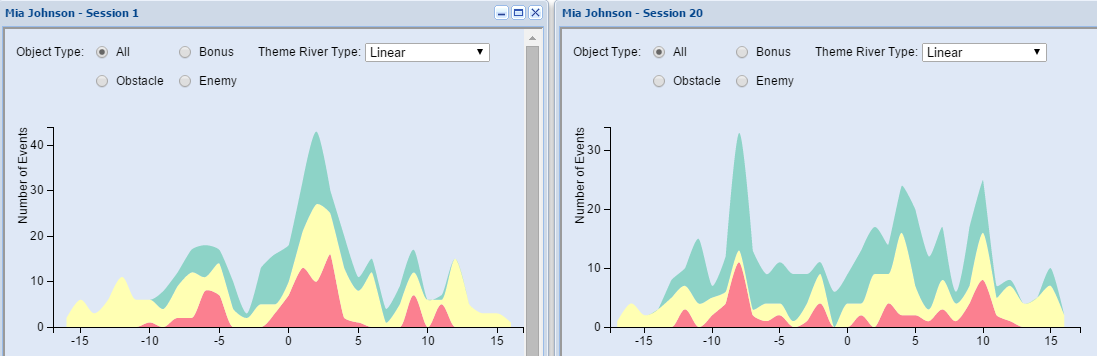
\includegraphics[width=140mm]{appendix_case1_compare_session_stackedgraph.png}
\caption{Stacked Graph comparison of Session 1 and Session 20 played by healthy player}
\label{fig:app1_stacked}
\end{figure}

\begin{figure}[H]
\centering
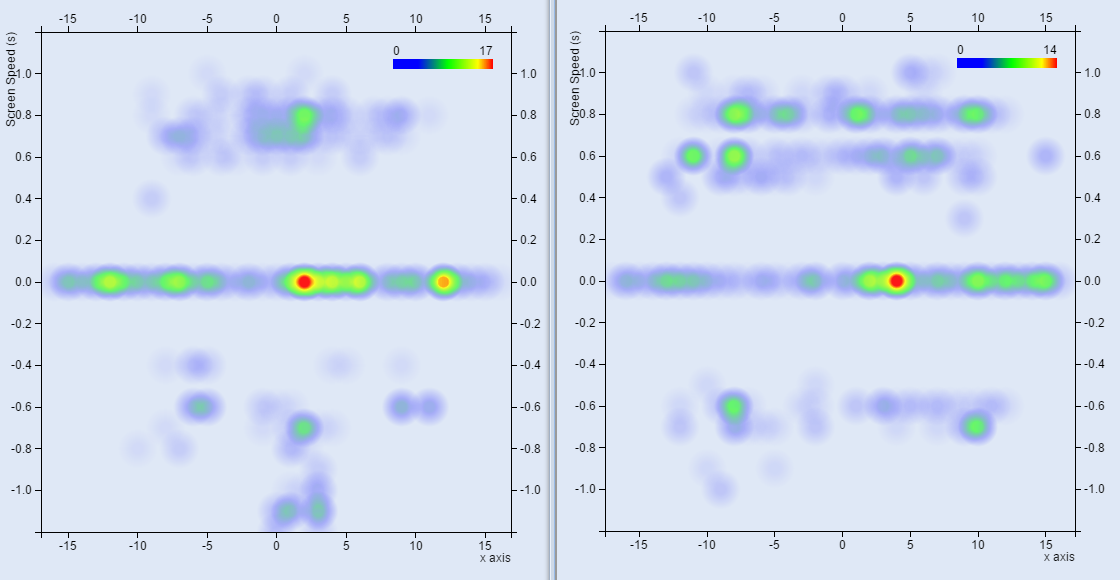
\includegraphics[width=140mm]{appendix_case1_compare_session_heatmap.png}
\caption{Heatmap comparison of Session 1(left) and Session 20(right) played by healthy player}
\label{fig:app1_heatmap}
\end{figure}
At first glance on Figure \ref{fig:app1_heatmap}, it is noticeable that there are more spot on the top part of the right heatmap (positive events) and less spot on the bottom part of the right heatmap (negative events). It also can be concluded that the player is able to control the boat well on the right chart since there are less spot with high speed of the negative events\ref{t12}. Which means that the player are getting better on playing the game. 

Focusing on events for Enemy \ref{t13} as shown in Figure \ref{fig:app1_stacked_enemy}, at a glance we can see that there are more negative events and very little positive events on the first session. While on session 20, there are less negative events and more positive events. This supports the conclusion made previously that the player has gotten better performance over time. Similar notes are depicted by Figure \ref{fig:app1_heatmap_enemy}. Here, on the right heatmap, there are more negative events which happened at faster screen speed\ref{t14}. This supports the fact that first time player are usually confuse on which direction to move their body/hand to make the boat go faster or slower.

\begin{figure}[H]
\centering
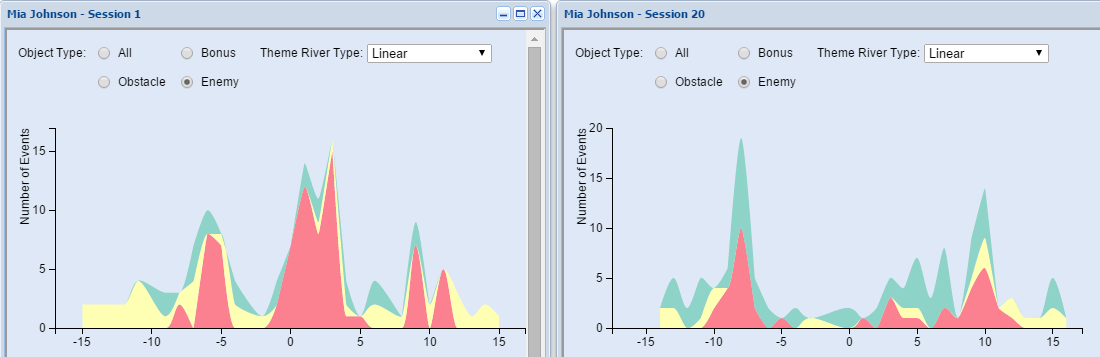
\includegraphics[width=140mm]{appendix_case1_compare_session_stackedgraph_enemy.png}
\caption{Stacked Graph comparison of Session 1 and Session 20 for Enemy played by healthy player}
\label{fig:app1_stacked_enemy}
\end{figure}

\begin{figure}[H]
\centering
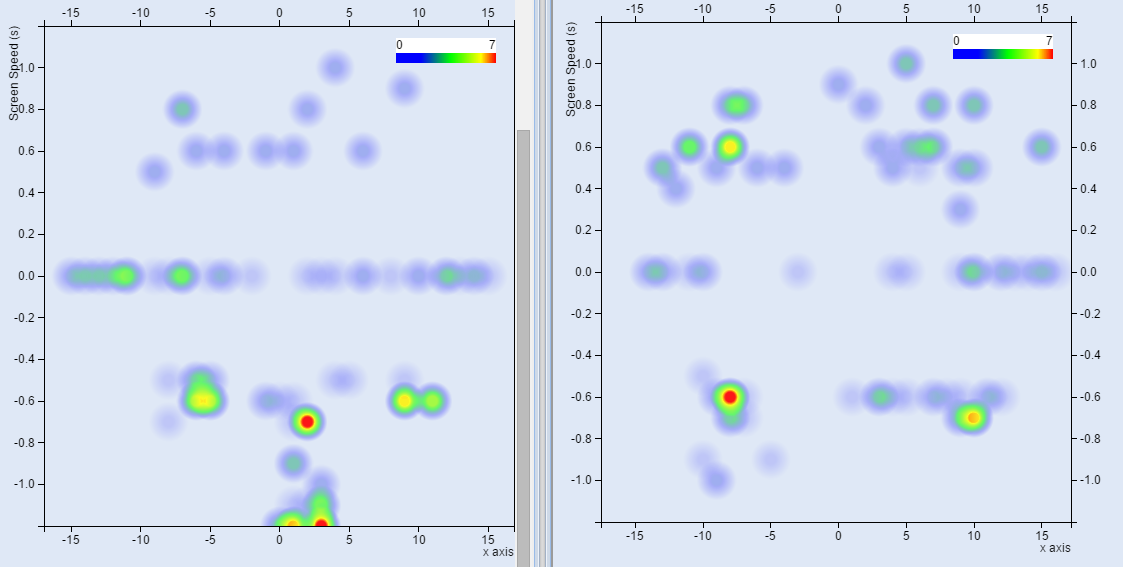
\includegraphics[width=140mm]{appendix_case1_compare_session_heatmap_enemy.png}
\caption{Heatmap comparison of Session 1(left) and Session 20(right) for Enemy played by healthy player}
\label{fig:app1_heatmap_enemy}
\end{figure}

The summary of all the session can be seen in Figure \ref{fig:case1_type1}. As we can see, the number of positive events are steadily increasing though fluctuate \ref{t21}. On session 19, there are very small number of negative events on all sections which indicate an improvement in the gameplay. 
\begin{figure}[H]
\centering
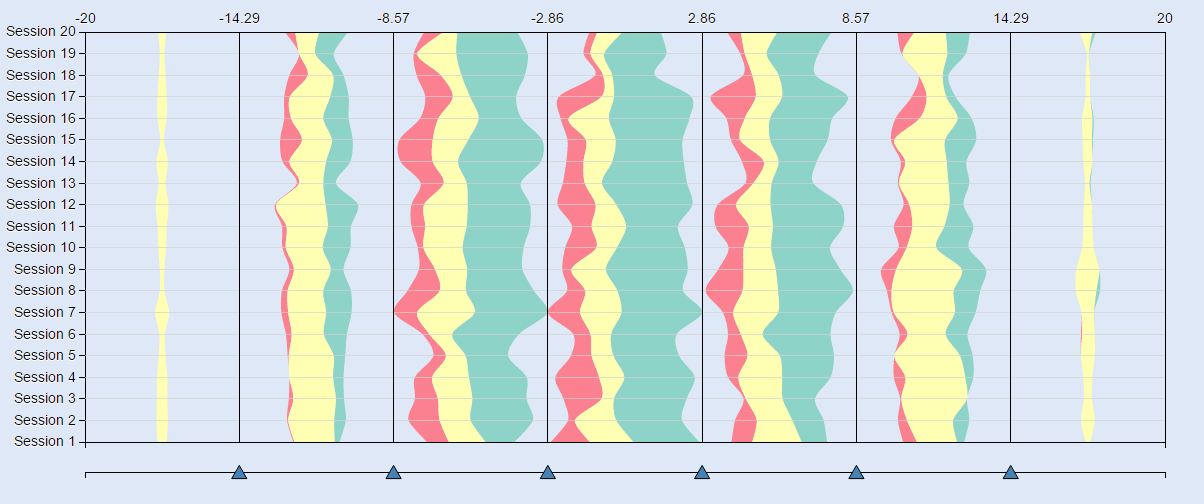
\includegraphics[width=140mm]{case1_type1.png}
\caption{Summary Visualization by x-range, played by healthy player}
\label{fig:case1_type1}
\end{figure}
In Figure \ref{fig:case1_type1_select}, we can see the evolution of the positive events \ref{t22}. Overall, the number are steady except for a certain session. However, on the right most section there are some positive events can be found which indicates that overtime, the player move more to the right. From Figure \ref{fig:case1_type2} we can conclude that the movement are more concentrated in the middle area of the screen [\ref{t23}\ref{t24}].

In Figure \ref{fig:case1_clustered}, two clustered sections are presented. In Figure \ref{4merged} left, we can see that all three sections (12-13, 13-14, 14-15) are similar in which each one of them has a little positive events on the lower half of the sections. Section 15-16 is similar to section 14-15 in term of the proportion as well as the evolution of neutral events. Therefore, these four sections are merged together forming one sections on the right\ref{t25}. Similarly, in Figure \ref{3merged}, we can see that all three sections has similar proportion of negative, neutral and positive events as well as similar evolution of each event type throughout the session. Thus forming one section on the right\ref{t25}.

\setlength{\intextsep}{0.5cm}
\begin{figure}[H]
\centering
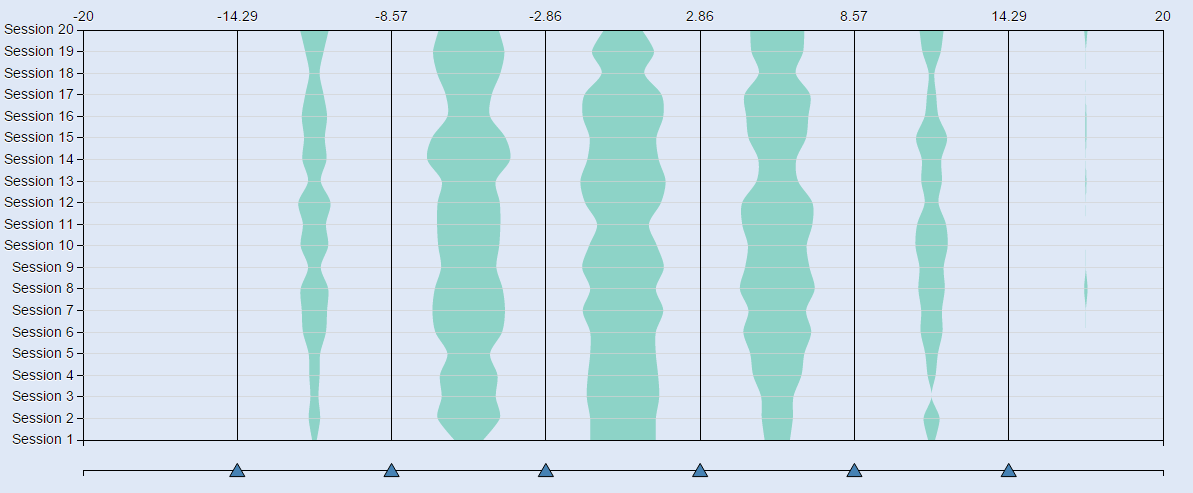
\includegraphics[width=140mm]{case1_type1_select.png}
\caption{Summary Visualization by x-range, filtered for positive events, played by healthy player}
\label{fig:case1_type1_select}
\vspace{1cm}
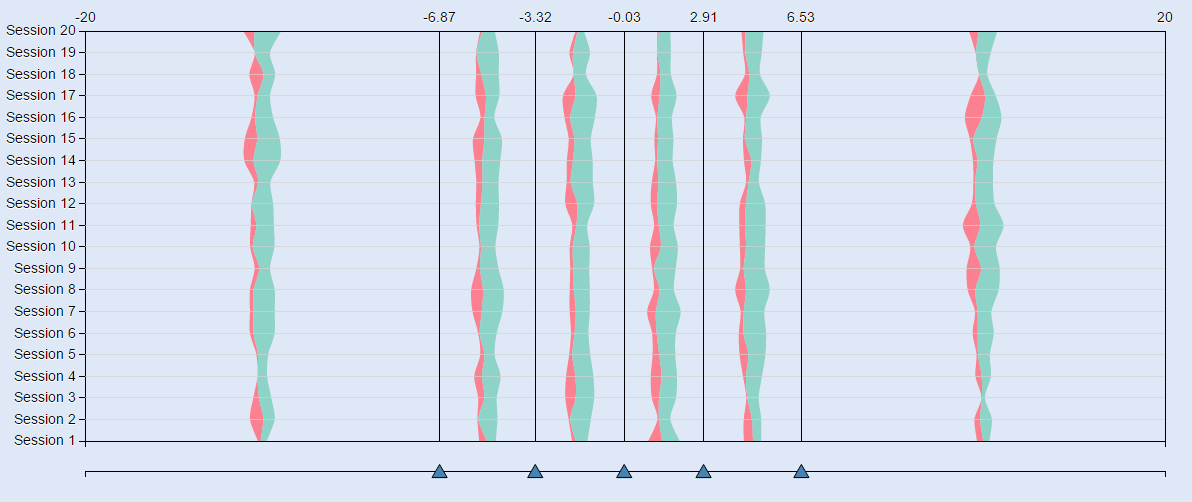
\includegraphics[width=140mm]{case1_type2.png}
\caption{Summary Visualization by number of events, filtered for positive and negative events, played by healthy player}
\label{fig:case1_type2}
\end{figure}

\begin{figure}[H]%
    \centering
    \subfloat[4 sections merged, threshold 0.22]{{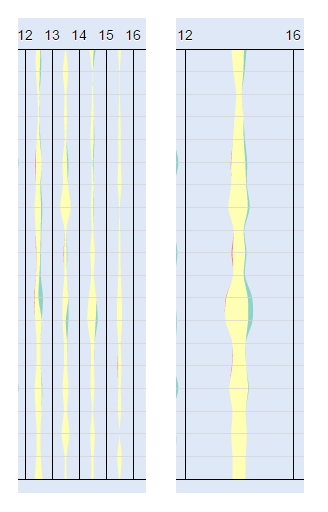
\includegraphics[scale=0.7]{case1_cluster1.png} 
    \label{4merged}}}%
    \qquad
    \subfloat[3 sections merged, threshold 0.26]{{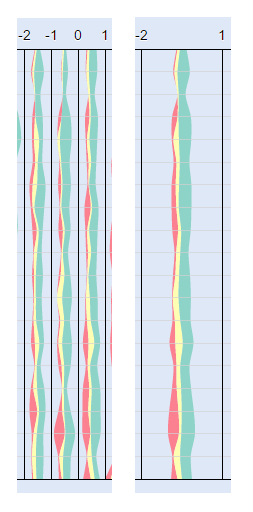
\includegraphics[scale=0.7]{case1_cluster2.png}
    \label{3merged} }}%
    \caption{Summary Visualization by clustering, played by healthy player}%
    \label{fig:case1_clustered}%
\end{figure}

\section{Case Study 2: Patient}
We have several patient data set, however most of these data set have very small number of session. Thus for the second case study, we chose data set from patient with enough sessions so that we can confirm the functionality of the developed visualization interface. Consequently, log files of game played by Patient 6 is used for this case study. There are 15 sessions which are played over the course of three weeks. However, these sessions are of two game type: HANDPOINT (6 sessions) and BODYTILT (9 session). Here, only the sessions of HANDPOINT exercise will be discussed. The game for this patient is set to show only obstacles and bonuses.

Focusing on the second session of HANDPOINT shown in Figure \ref{fig:case2_stacked}, it can be seen that the positive and negative events only appear on the right half of the chart indicating that the player only move to the right \ref{t11}. The yellow area are bigger compared to the green and red areas, showing that there are a lot of missed/avoided objects. 

From Figure \ref{fig:case2_heatmap}, we can see that there are many neutral events on the left side of the screen. While positive and negative events are happened only on the right side with similar screen speed indicating that the player didn't change the pace of the game \ref{t12}. Figure \ref{fig:case2_stacked_bonus} and \ref{fig:case2_heatmap_bonus} shows events related to bonus \ref{t13}\ref{t14}. Therefore, there are only positive and neutral events. Here, it can be seen that on the far right, there are no bonus is missed, however, on the left side all bonuses are missed. Based on these charts, we may conclude that the player has some difficulty to move to the left. It's important to see if this is an isolated case or happened all the time. Therefore, we need to see the pattern of movement for all sessions which will be discussed shortly.
\begin{figure}[H]
\centering
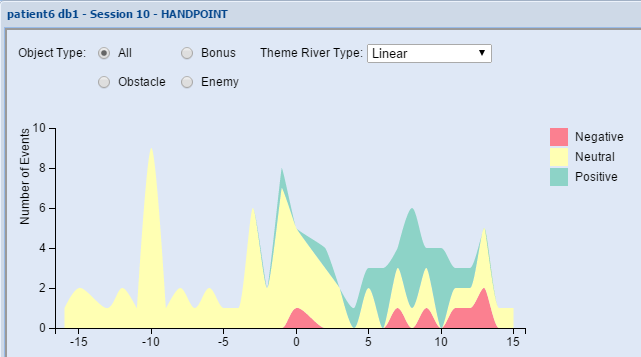
\includegraphics[width=120mm]{case2_stacked.png}
\caption{Stacked Graph of Patient 6 on second session}
\label{fig:case2_stacked}
\vspace{1cm}
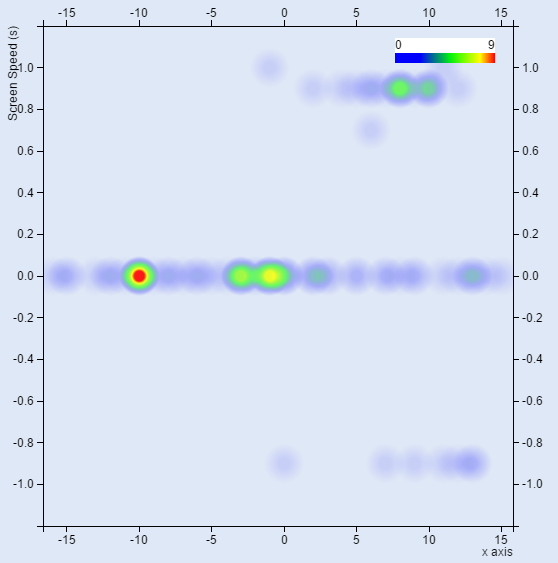
\includegraphics[width=90mm]{case2_heatmap.png}
\caption{Heatmap of Patient 6 on second session}
\label{fig:case2_heatmap}
\end{figure}

\begin{figure}[H]
\centering
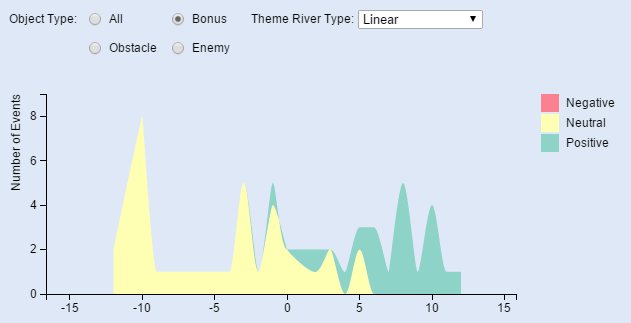
\includegraphics[width=120mm]{case2_stacked_bonus.png}
\caption{Stacked Graph of Patient 6 on second session, filtered by bonus}
\label{fig:case2_stacked_bonus}
\vspace{1cm}
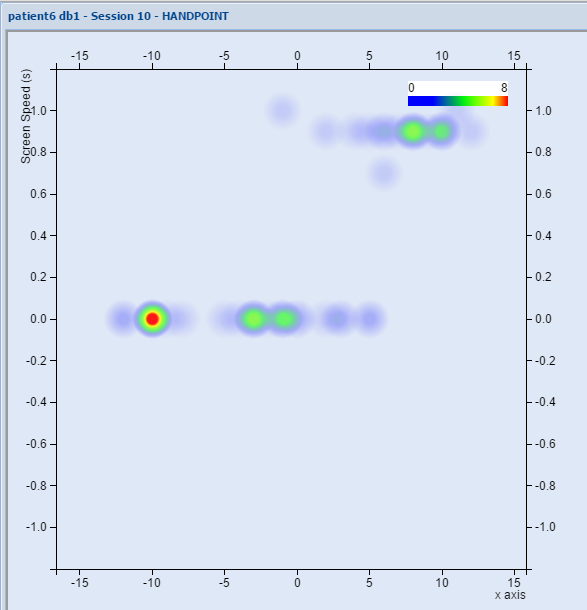
\includegraphics[width=90mm]{case2_heatmap_bonus.png}
\caption{Heatmap of Patient 6 on second session, filtered by bonus}
\label{fig:case2_heatmap_bonus}
\end{figure}

The summary visualization shown in Figure \ref{fig:case2_summary} confirmed that for 4 sessions, the player only move to the right side. If the -2.29 line is dragged to the right, the red and green area only appears from -1.96 boundary. However, from the fifth sessions, there are movements on the left side indicated by a small number of negative and positive events \ref{t21}. Figure \ref{fig:case2_summary_neutral} shows the evolution of neutral events \ref{t22}. Here, we can see that there are more neutral events on the left side compared to the right throughout all sessions. In Figure \ref{fig:case2_clustered}, two clustered sections are presented. In Figure \ref{case2_2merged} left, we can see that both sections have similar neutral event evolution. Hence, the sections are merged together forming one sections on the right\ref{t25}. Similarly, in Figure \ref{case2_4merged}, we can see that consecutive sections have similar neutral events evolution. Thus forming one section on the right\ref{t25}. Consistent with all the previous visualization, Figure \ref{fig:case2_summary_type2} shows that the movements are concentrated more on the right side [\ref{t23}\ref{t24}].

\begin{figure}[H]
\centering
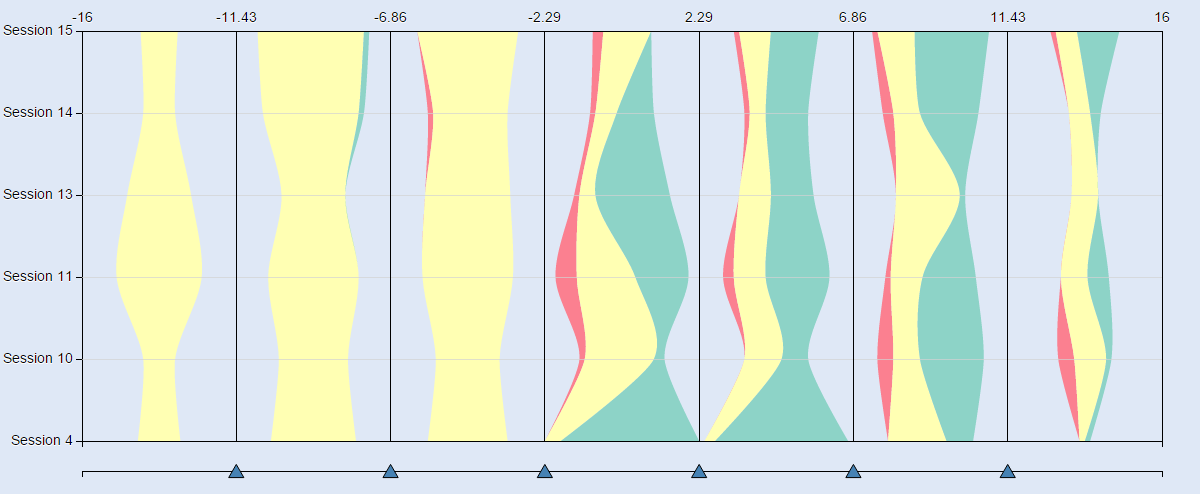
\includegraphics[width=140mm]{case2_summary.png}
\caption{Summary visualization of Patient 6}
\label{fig:case2_summary}
\vspace{1cm}
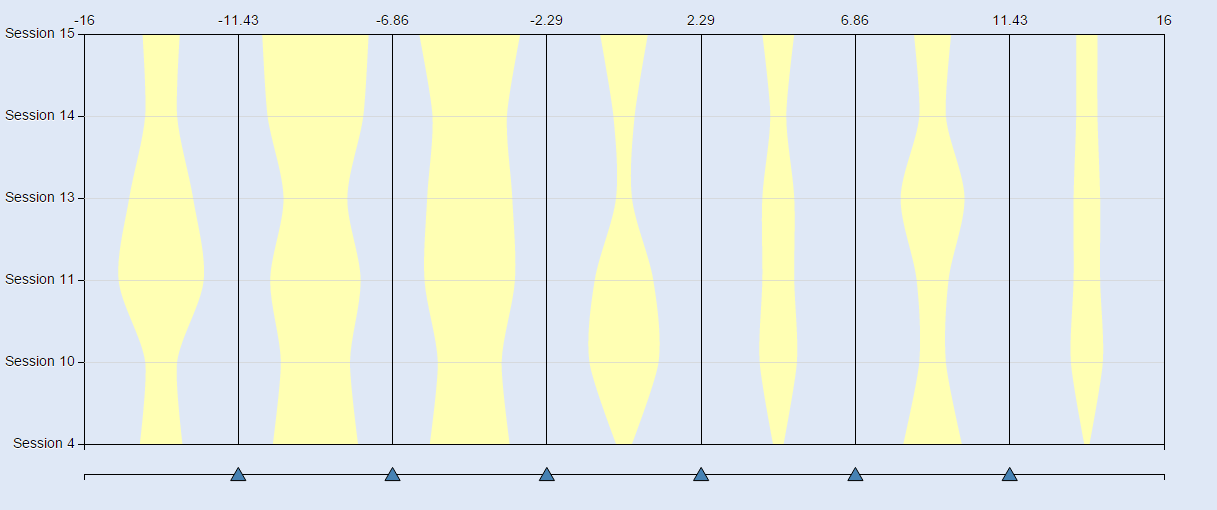
\includegraphics[width=140mm]{case2_summary_neutral.png}
\caption{Summary visualization of Patient 6, filtered by neutral events}
\label{fig:case2_summary_neutral}
\end{figure}

\begin{figure}[H]%
    \centering
    \subfloat[2 sections merged, threshold 0.05]{{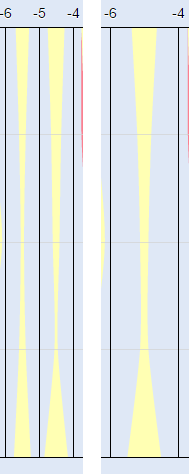
\includegraphics[scale=0.6]{case2_cluster1.png} 
    \label{case2_2merged}}}%
    \qquad
    \subfloat[4 sections merged, threshold 0.09]{{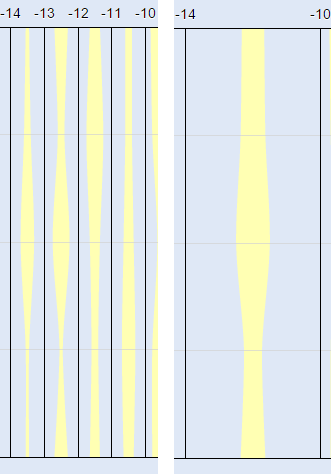
\includegraphics[scale=0.6]{case2_cluster2.png}
    \label{case2_4merged} }}%
    \caption{Summary visualization of Patient 6, clustered}%
    \label{fig:case2_clustered}%
    \vspace{1cm}
    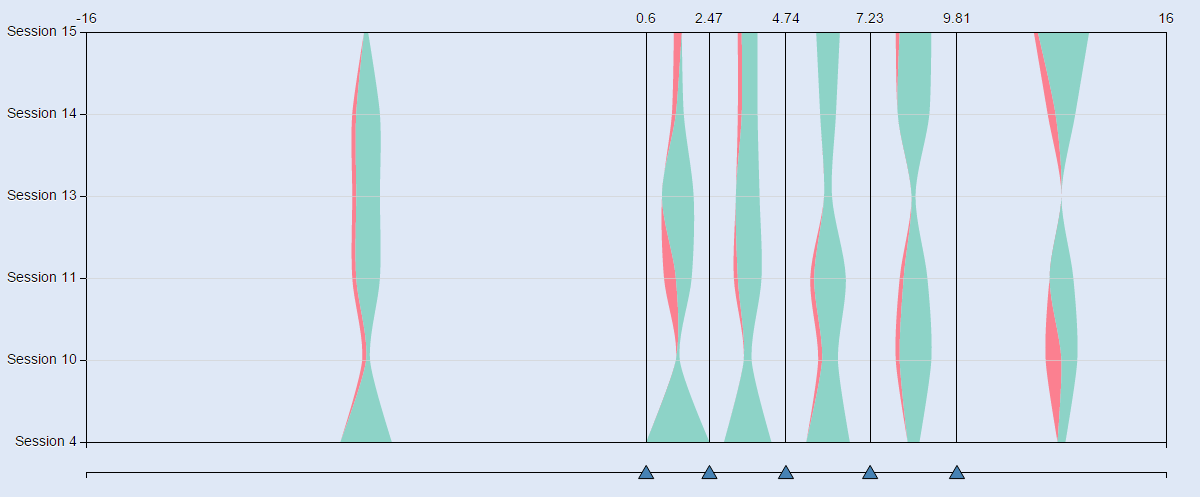
\includegraphics[width=140mm]{case2_summary_type2.png}
	\caption{Summary visualization of Patient 6 with sections divided by number of events, filtered by positive and negative events}
	\label{fig:case2_summary_type2}
\end{figure}

Movement of person with pathology are highly affected by the type of pathology. On the second case study, throughout all sessions the movements are concentrated to the right side with almost no movement on the left side. Therefore we can assume that the patient has his left side of the body affected. While for healthy person, the movement are more spread out on both left and right side with more concentration in the middle.
